\documentclass[11pt]{article}
\usepackage{amsmath,amssymb,amsthm}
\usepackage{tabu}
\usepackage{graphicx}
%\usepackage[bw]{mcode}
\usepackage[margin=.6in]{geometry}
\usepackage{tikz}
\usepackage{float}
\usepackage{textcomp}
\usepackage{multicol}
\addtolength{\topmargin}{.5in}
\usepackage{fancyhdr}
\setlength{\parindent}{0pt}
\setlength{\parskip}{5pt plus 1pt}
\setlength{\headheight}{20pt}
\renewcommand{\headrulewidth}{0pt}
\setlength{\headheight}{30.0pt}
\newcommand\question[2]{\vspace{.25in}\hrule\textbf{#1: #2}\vspace{.5em}\hrule\vspace{.10in}}
\renewcommand\part[1]{\vspace{.10in}\textbf{(#1)}}
\newcommand\enter{\vspace{.50in}}
\newcommand\algorithm{\vspace{.10in}\textbf{Algorithm: }}
\newcommand\correctness{\vspace{.10in}\textbf{Correctness: }}
\newcommand\runtime{\vspace{.10in}\textbf{Running time: }}
\pagestyle{fancyplain}

\begin{document}\raggedright
\newcommand\Page{\page  / \lastPage}
\newcommand\page{1}
\newcommand\qN[2]{\Large {#1} \small{#2} \normalsize}

% info
\newcommand\name{Ashley}
\newcommand\lastName{Gannon}
\newcommand\dueDate{September 3rd, 11:59PM}
\newcommand\hwnum{1}
\newcommand\ExNum{   }

\newcommand\lastPage{3}

% set info
\lhead{\large Homework \hwnum }
\rhead{\rightHead}
\chead{\LARGE{Unix Command-Line Interface}}
\newcommand\rightHead{\large Due Sep 3 11:59PM}

%Section B==============Put your answers to the questions below here=======================
%\includegraphics[width = 4in]{Graph2}
%tabular with tabu package
%\begin{lstlisting}
%\end{lstlisting}

\question{1}{Binary representation of decimal (20 pts)}
Determine the binary numbers which represent the following integers:
\begin{figure}[H]
    \center
    \begin{tikzpicture}
        \node[right] at (0,0) {};
        \node[right] at (-16,0) {$11_{10}$:};
        \node[right] at (-16,-2) {$1100_{10}$:};
        \node[right] at (-16,-4) {$293_{10}$:};
        \node[right] at (-16,-6) {$97_{10}$:};
    \end{tikzpicture}
\end{figure}
\textbf{Show all work for credit.}
\vspace{0.5cm}

\question{2}{Decimal representation of binary (20 pts)}
Determine the decimal numbers which represent the following binary numbers:
\begin{figure}[H]
	\center
	\begin{tikzpicture}
	\node[right] at (0,0) {};
	\node[right] at (-16,0) {$1001011_{2}$:};
	\node[right] at (-16,-2) {$110001_{2}$:};
	\node[right] at (-16,-4) {$10101110_{2}$:};
	\node[right] at (-16,-6) {$10_{2}$:};
	\end{tikzpicture}
\end{figure}
\textbf{Show all work for credit.}
\vspace{0.5cm}

\newpage
\question{3}{Unix environment (10 pts)}
Below is a diagram of the Unix environment. In your own words please do the
following: list the three essential pieces of hardware on a computer (5pts);
describe the purpose of the kernel (5pts); describe the purpose of the shell (5pts); give at least three examples of applications or utilities (5pts). \\[0.5cm]
\begin{figure}[H]
    \center
    \scalebox{.8}{
    \begin{tikzpicture}
        \draw [black, thick] (0,0) circle [radius=1];
        \draw [black, thick] (0,0) circle [radius=2];
        \draw [black, thick] (0,0) circle [radius=3];
        \draw [black, thick] (0,0) circle [radius=4];
        \draw [thick] (0.3,0) --(6,0);
        \draw [thick] (1,1) --(4,3) --(5,3);
        \draw [thick] (1.75,-1.75) --(4,-3) --(5,-3);
        \draw [thick] (-3.5,0) --(-6,0) --(-7.5,-1);
        \node[] at (7,0.05) {Hardware:};
        \node[] at (6,3.05) {Kernel:};
        \node[] at (6,-2.95) {Shell:};
        \node[] at (-8,-1.45) {Applications/Uilities:};
    \end{tikzpicture}}
\end{figure}

\newpage
\question{4}{Unix special symbols (10 pts)}
Define the special meaning of the following symbols in the Unix terminal when
specifying paths to directories or files:
\begin{figure}[H]
    \center
    \begin{tikzpicture}
        \node[] at (0,0) {};
        \node[right] at (-16,-0) {the `$\sim$' symbol:};
        \node[right] at (-16,-1) {the `.' symbol:};
        \node[right] at (-16,-2) {the `..' symbol:};
        \node[right] at (-16,-3) {the `$\ast$' symbol:};
    \end{tikzpicture}
\end{figure}

\question{5}{Unix commands (20 points)}
Describe the main purpose of each of the following commands or characters if
used on the command-line:
\begin{figure}[H]
	\center
	\begin{tikzpicture}
	\node[right] at (0,0) {};
	\node[right] at (-16,0) {$\texttt{cat}$:};
	\node[right] at (-16,-1.5) {$\texttt{mv}$:};
	\node[right] at (-16,-3) {$\texttt{cp}$:};
	\node[right] at (-16,-4.5) {$\texttt{grep}$:};
	\node[right] at (-16,-6) {$\texttt{ls}$:};
	\node[right] at (-16,-7.5) {$\texttt{pwd}$:};
	\node[right] at (-16,-9) {$\texttt{cd}$:};
	\end{tikzpicture}
\end{figure}

\newpage
\question{6}{Unix commands (20 pts)}
Suppose you are given three files, \texttt{file1.txt}, \texttt{file2.txt} and
\texttt{file3.txt}, containing text, shown below using the \texttt{cat} command
(note that the \texttt{\$} symbol simply indicates a command prompt, as opposed
to command output):
\begin{multicols}{3}
    { \footnotesize 
    \texttt{\$ cat file1} \\
    \texttt{At Bell Laboratories} \\
    \texttt{UNIX systems provide} \\
    }
    \columnbreak
    { \footnotesize 
    \texttt{\$ cat file2} \\
    \texttt{more timesharing ports} \\
    }
    \columnbreak
    { \footnotesize 
    \texttt{\$ cat file3} \\
    \texttt{than all other systems} \\
    }
\end{multicols}
Suppose now that you execute the following command in your terminal:
\begin{figure}[H]
    \center
    \begin{tikzpicture}
        \node[] at (0,0) {};
        \node[right] at (-16,0) {\footnotesize \texttt{\$ cat file2 file3 > file1}};
    \end{tikzpicture}
\end{figure}
Please write the expected output of the following command:
\begin{figure}[H]
    \center
    \begin{tikzpicture}
        \node[] at (0,0) {};
        \node[right] at (-16,0) {\footnotesize \texttt{\$ cat file1}};
    \end{tikzpicture}
\end{figure}
\vspace{0.5cm}
\vspace{0.5cm}
\vspace{0.5cm}
Use the \texttt{touch} command to make \texttt{file1.txt}, \texttt{file2.txt} and
\texttt{file3.txt}. You may add the above sentences using vim or by opening the \texttt{.txt} files with a text editor. Check your work on your machine!


\newpage
\renewcommand\page{2}
\renewcommand\rightHead{\lastName \\ \Page}
\chead{MCMC in Tree Space}
\setlength{\headheight}{13pt}

\setlength{\headheight}{13pt}
\newpage
\renewcommand\page{3}

\setlength{\headheight}{13pt}
\newpage
\renewcommand\page{4}

\end{document}
